Consider the empirical risk from above. The Hessian matrix w.r.t.\,to a flattening scheme $\vec$ is given by
\begin{align*}
  \hess_{\vtheta}^{\vec} \gL_{\sD}(\vtheta)
  =
  R
  \sum_{n=1}^N
  \hess_{\vtheta}^{\vec} \ell_n(\vtheta) \in \sR^{D \times D}\,.
\end{align*}
and contains the second-order partial derivatives of $\gL_{\sD}(\vtheta)$, that is
\begin{align*}
  [\hess_{\vtheta}^{\vec} \gL_{\sD}(\vtheta)]_{i,j}
  =
  \frac{\partial^2 \gL_{\sD}(\vtheta)}{\partial [\vec(\vtheta)]_i \partial [\vec(\vtheta)]_j}\,.
\end{align*}

\switchcolumn[1]*
\begin{figure}
  \centering
  \begin{minipage}[t]{0.495\linewidth}
    \centering
    $\cvec$\vspace{1ex}
    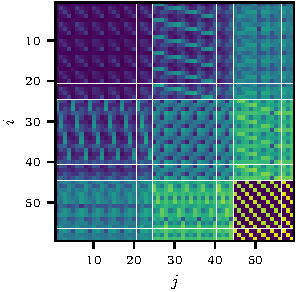
\includegraphics[width=\linewidth]{../kfs/plots/synthetic_cvec_hessian.pdf}
  \end{minipage}
  \hfill
  \begin{minipage}[t]{0.495\linewidth}
    \centering
    $\rvec$\vspace{1ex}
    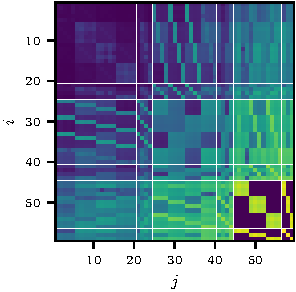
\includegraphics[width=\linewidth]{../kfs/plots/synthetic_rvec_hessian.pdf}
  \end{minipage}
  \\
  \begin{minipage}[t]{0.495\linewidth}
    \centering
    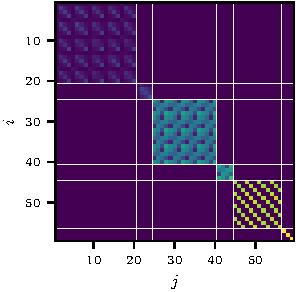
\includegraphics[width=\linewidth]{../kfs/plots/synthetic_cvec_hessian_bda.pdf}
  \end{minipage}
  \hfill
  \begin{minipage}[t]{0.495\linewidth}
    \centering
    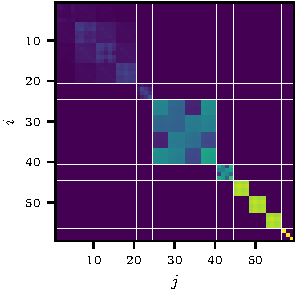
\includegraphics[width=\linewidth]{../kfs/plots/synthetic_rvec_hessian_bda.pdf}
  \end{minipage}
  \caption{Visualization of the Hessian and its block-diagonal approximation using different flattening schemes.
    Hessian blocks are visually highlighted with white lines.
    Left column uses $\rvec$-flattening, right column uses $\cvec$-flattening.
    The Hessian was evaluated on synthetic data ($N=100$) using an MLP with three fully-connected layers and ReLU activations (5-4-4-3, our notation considers applying the weight matrix and adding the bias as two layers, hence $L=6$) and square loss.
  }
\end{figure}

\switchcolumn[0]

Due to the tuple/list structure of $\vtheta$, the Hessian has a block structure.
Using the shorthands $\hess_{i,j}^{\vec} \gL \coloneq \hess_{\vtheta^{(i)}, \vtheta^{(j)}}^{\vec} \gL_{\sD}(\vtheta)$
which contains mixed second-order partial derivatives w.r.t.\,$\vtheta^{(i)}$ and $\vtheta^{(j)}$, as well as the shorthand $\hess_{i}^{\vec} \gL \coloneq \hess_{\vtheta^{(i)}}^{\vec} \gL_{\sD}(\vtheta)$, we can write the Hessian as
\begin{align*}
  \hess_{\vtheta}^{\vec} \gL
  =
  \begin{pmatrix}
    \hess_1^{\vec} \gL
    &
      \hess_{1, 2}^{\vec} \gL
    &
      \cdots
    &
      \hess_{1, L}^{\vec} \gL
    \\
    \hess_{2, 1}^{\vec} \gL
    &
      \hess_2^{\vec} \gL
    &
      \cdots
    &
      \hess_{2, L}^{\vec} \gL
    \\
    \vdots & \cdots & \ddots & \vdots
    \\
    \hess_{L, 1}^{\vec} \gL
    &
      \hess_{L, 2}^{\vec} \gL
    &
      \cdots
    &
      \hess_L^{\vec} \gL
  \end{pmatrix}\,.
\end{align*}
In the following, we will only consider the block diagonal approximation of this matrix,
\begin{align*}
  \tilde{\hess}_{\vtheta}^{\vec} \gL
  =
  \begin{pmatrix}
    \hess_1^{\vec} \gL & \vzero & \cdots & \vzero
    \\
    \vzero & \hess_2^{\vec} \gL & \ddots & \vdots
    \\
    \vdots & \ddots & \ddots & \vzero
    \\
    \vzero & \cdots & \vzero & \hess_L^{\vec} \gL
  \end{pmatrix}\,.
\end{align*}
i.e., individual blocks $\{ \hess_{\vtheta^{(i)}}^{\vec} \gL_{\sD}(\vtheta)\}$.
%%% Local Variables:
%%% mode: latex
%%% TeX-master: "../main"
%%% End:
